\documentclass{standalone}
\usepackage{tikz}
\usepackage{nicefrac}
\begin{document}

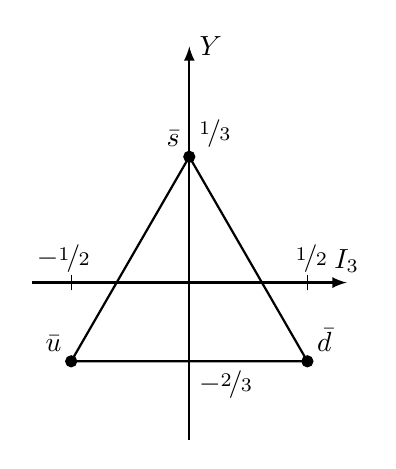
\begin{tikzpicture}

% Definir el tamaño del lado del triángulo equilátero
\def\side{3}

% Coordenadas de los vértices del triángulo equilátero (u, d, s)
\coordinate (d) at (-\side/2, 0);
\coordinate (u) at (\side/2, 0);
\coordinate (s) at (0, {sqrt(3)/2 * \side});


% Dibujar el triángulo equilátero
\draw[thick] (u) -- (d) -- (s) -- cycle;

% Colocar etiquetas para cada partícula
\node[above right] at (u) {$\bar{d}$};
\draw[fill=black] (u) circle (2pt);

\node[above left] at (d) {$\bar{u}$};
\draw[fill=black] (d) circle (2pt);


\node[above left] at (s) {$\bar{s}$};
\draw[fill=black] (s) circle (2pt);
\node[below right] at (0,0) {$-\nicefrac{2}{3}$};

%Ejes de la hipercarga e isospin
\draw[-latex, thick] (0,-1)--(0,4) node[right]{$Y$};
\draw[-latex, thick] (-2,1)--(2,1) node[above]{$I_3$};
\node[above] at(-\side/2-0.1,1){$-\nicefrac{1}{2}$};
\draw[fill=black] (-\side/2,1-0.1)--(-\side/2,1+0.1) ;
\node[above] at(\side/2+0.05,1){$\nicefrac{1}{2}$};
\draw[fill=black] (+\side/2,1-0.1)--(\side/2,1+0.1) ;
\node[above right] at(0,{\side*sqrt(3)/2}) {$\nicefrac{1}{3}$};

\end{tikzpicture}

\end{document}
